% Created 2013-07-03 Wed 13:27
\documentclass[11pt]{article}
\usepackage[utf8]{inputenc}
\usepackage[T1]{fontenc}
\usepackage{fixltx2e}
\usepackage{graphicx}
\usepackage{longtable}
\usepackage{float}
\usepackage{wrapfig}
\usepackage[normalem]{ulem}
\usepackage{textcomp}
\usepackage{marvosym}
\usepackage{wasysym}
\usepackage{latexsym}
\usepackage{amssymb}
\usepackage{amstext}
\usepackage{hyperref}
\tolerance=1000
\usepackage[comma, authoryear]{natbib}
\usepackage{subfig}
\usepackage{hyperref}
\hypersetup{
colorlinks,%
citecolor=black,%
filecolor=black,%
linkcolor=blue,%
urlcolor=black
}
\usepackage[french,frenchb]{babel}
\usepackage[compact]{titlesec}
\author{Martin Marier}
\date{}
\title{L'écriture électroacoustique pour interface tangible}
\hypersetup{
  pdfkeywords={},
  pdfsubject={},
  pdfcreator={Emacs 24.3.50.1 (Org mode 8.0.3)}}
\begin{document}

\maketitle

\section*{Introduction}
\label{sec-1}
Ce projet de thèse acomprend trois axes principaux: la conception d'une interface
musicale, la conception de mappages pour cette interface, ainsi que la
composition d'oeuvres électroacoustiques pour l'interface et les mappages
conçus.

Ladite interface est nommée l'\emph{éponge} et elle a l'allure d'un coussin rayé
(voir figure \ref{fig:eponge}).  Des capteurs en détectent les déformations
et un microcontrôleur achemine les données vers un ordinateur où les données
sont mappées sur des paramètres de synthèse et de traitement sonore.  Ce
dispositif permet l'interprétation de musiques électroacoustique devant
public.

\begin{figure}
  \centering
  \subfloat[]{\label{fig:epongeDroite}
    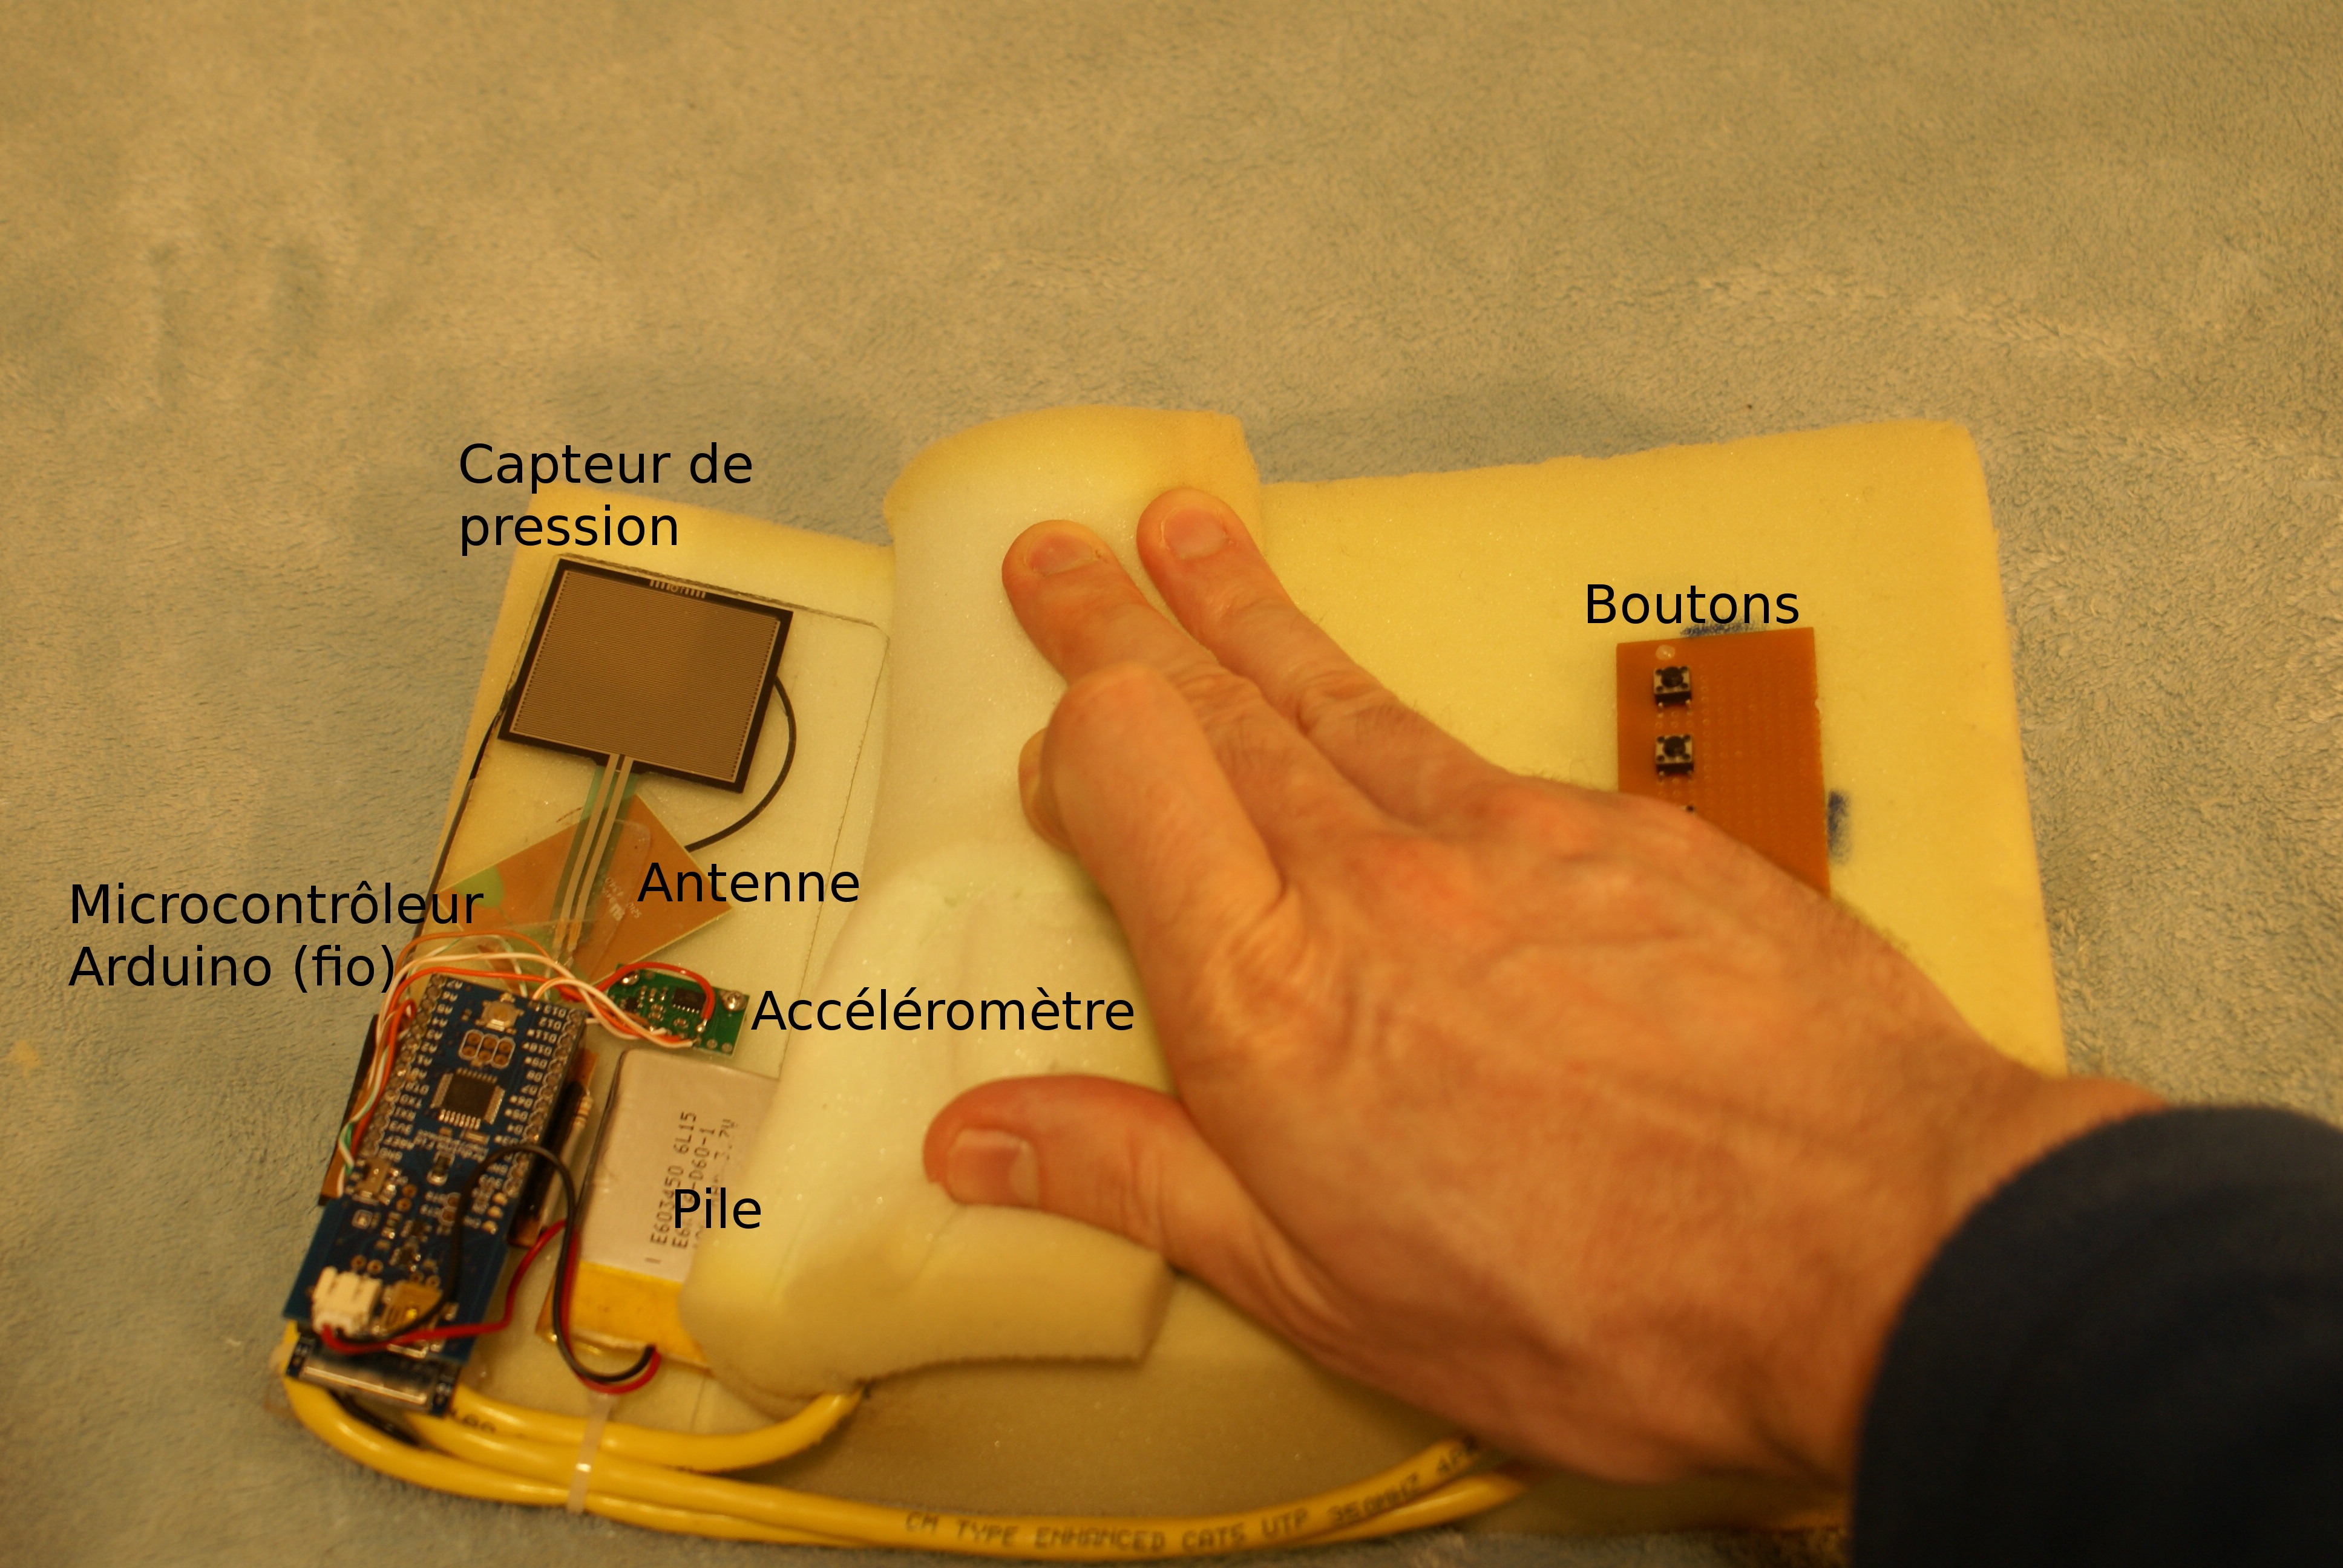
\includegraphics[height=0.14\textheight]{figs/spongeDroite.jpg}}
  \subfloat[]{\label{fig:epongeHousse}
    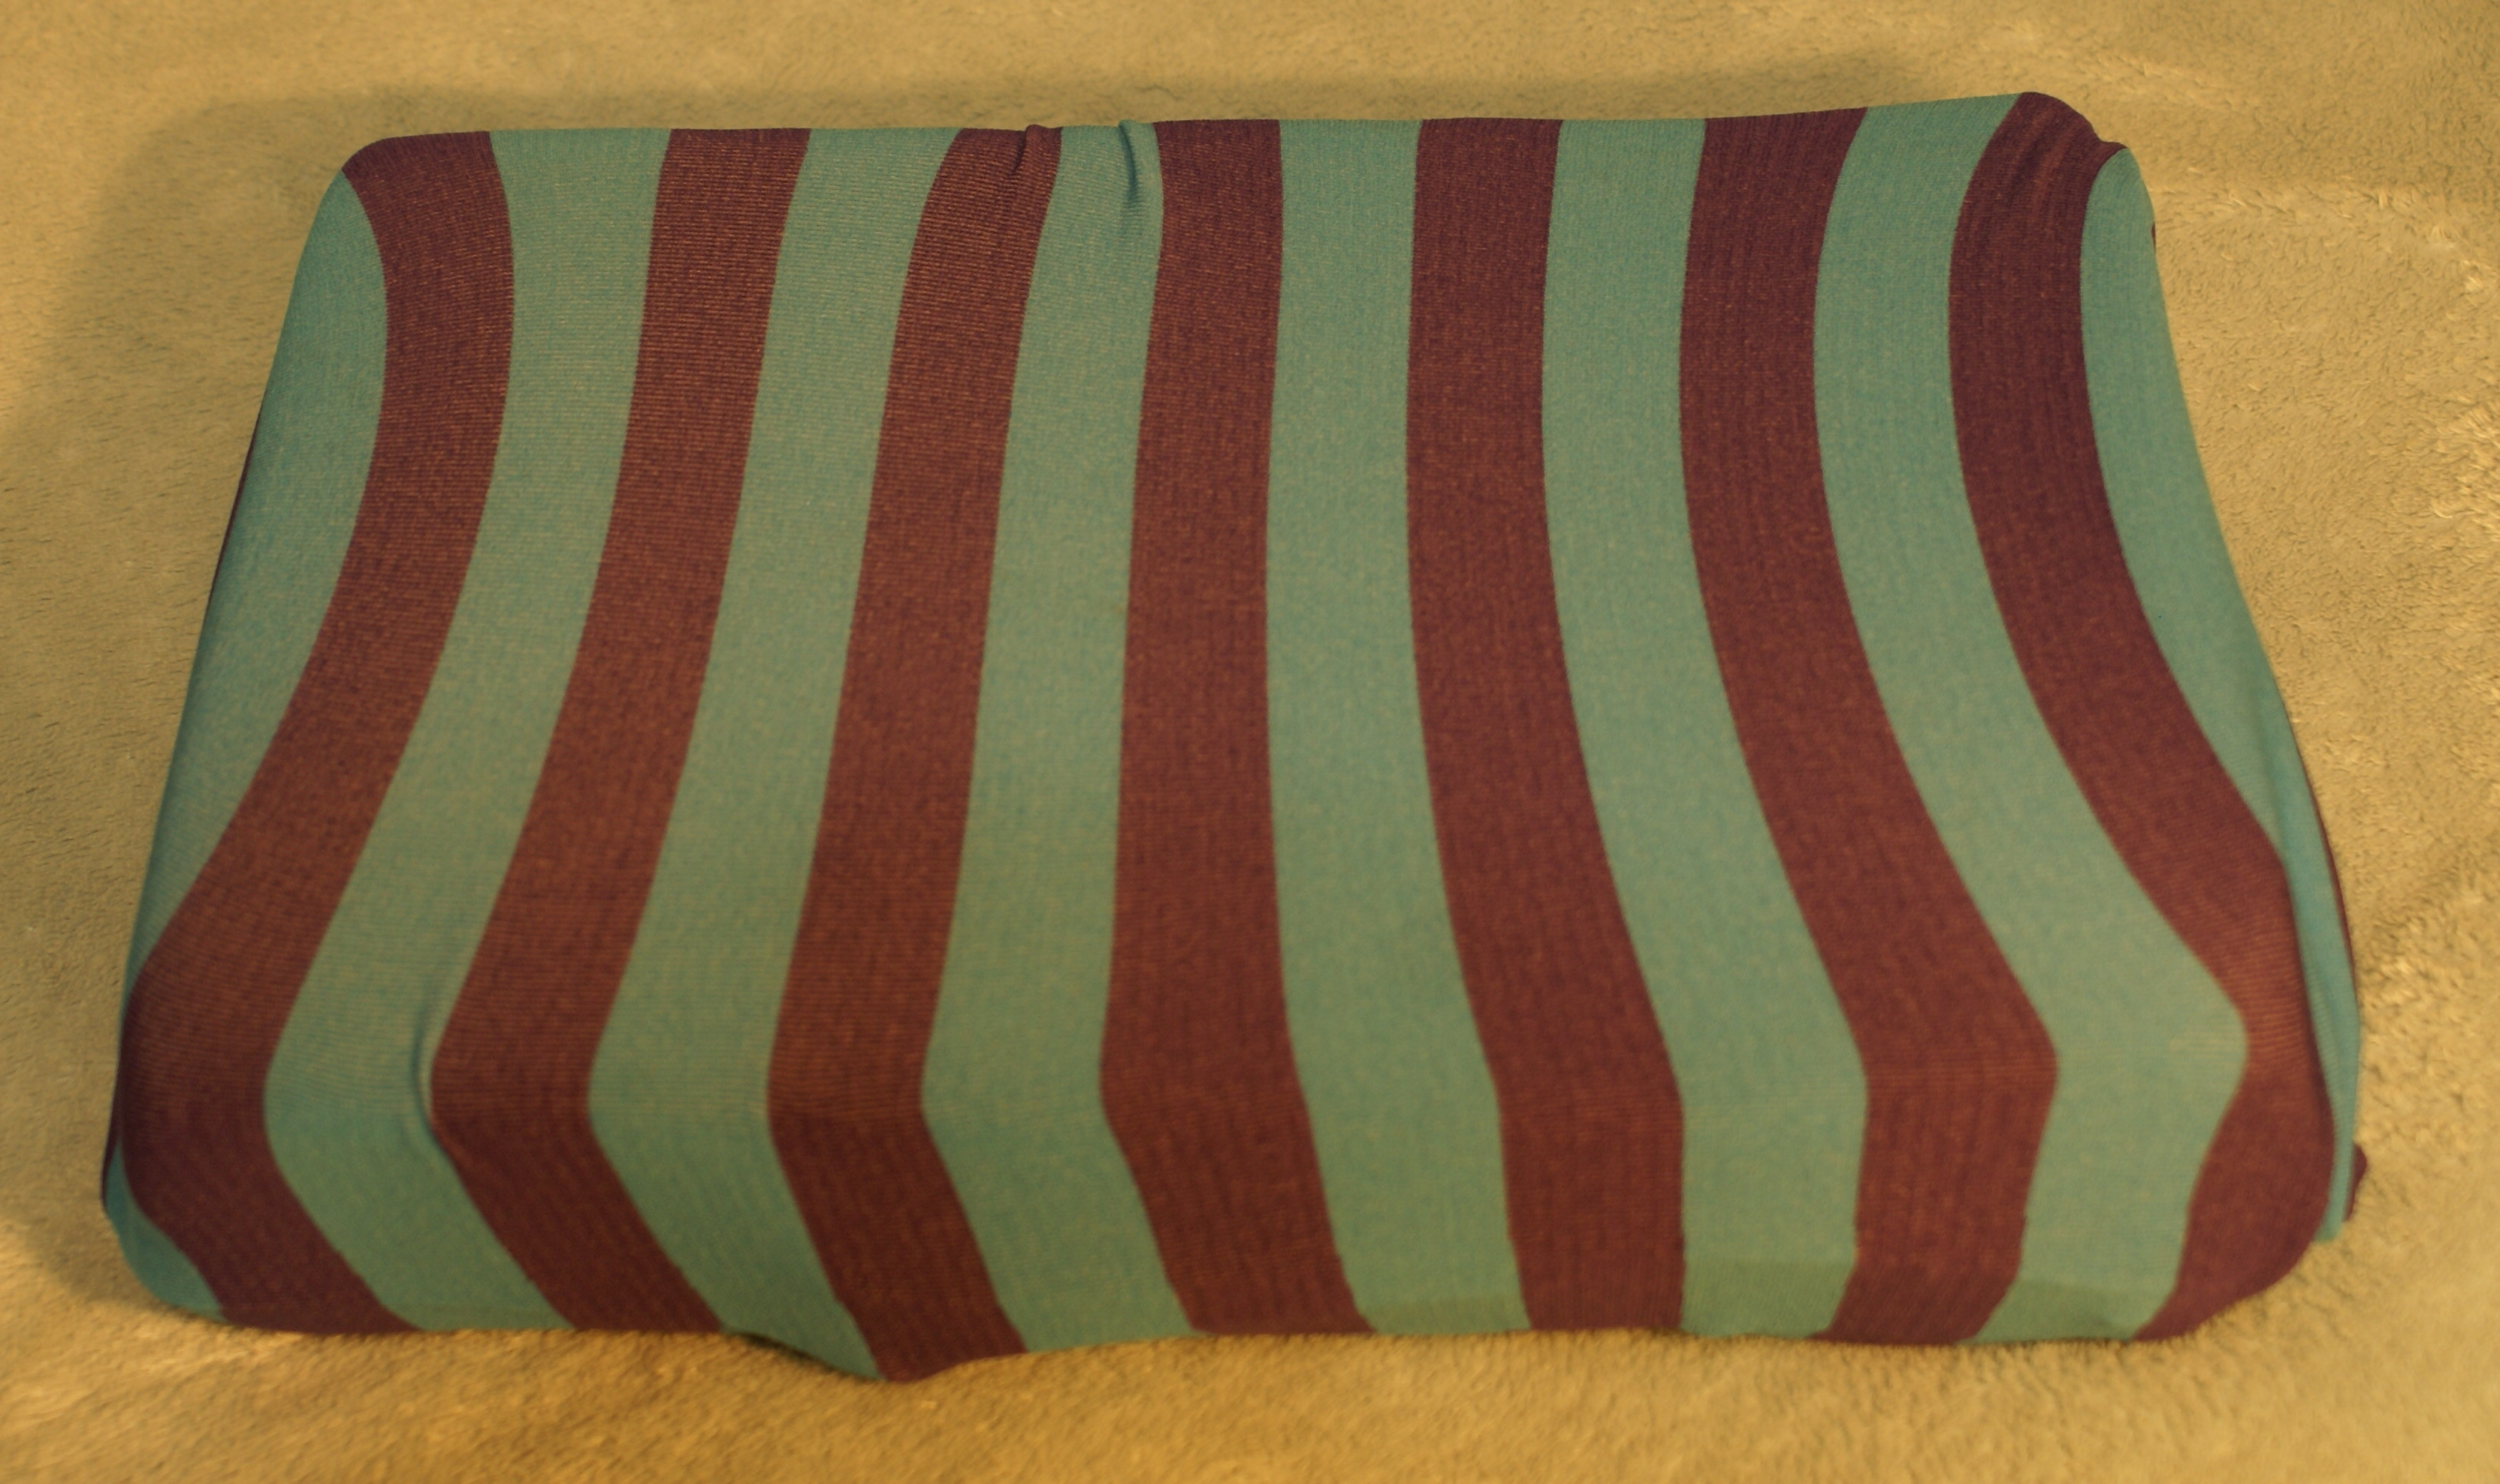
\includegraphics[height=0.14\textheight]{figs/spongeDressed.jpg}}
  \subfloat[]{\label{fig:epongeGauche}
    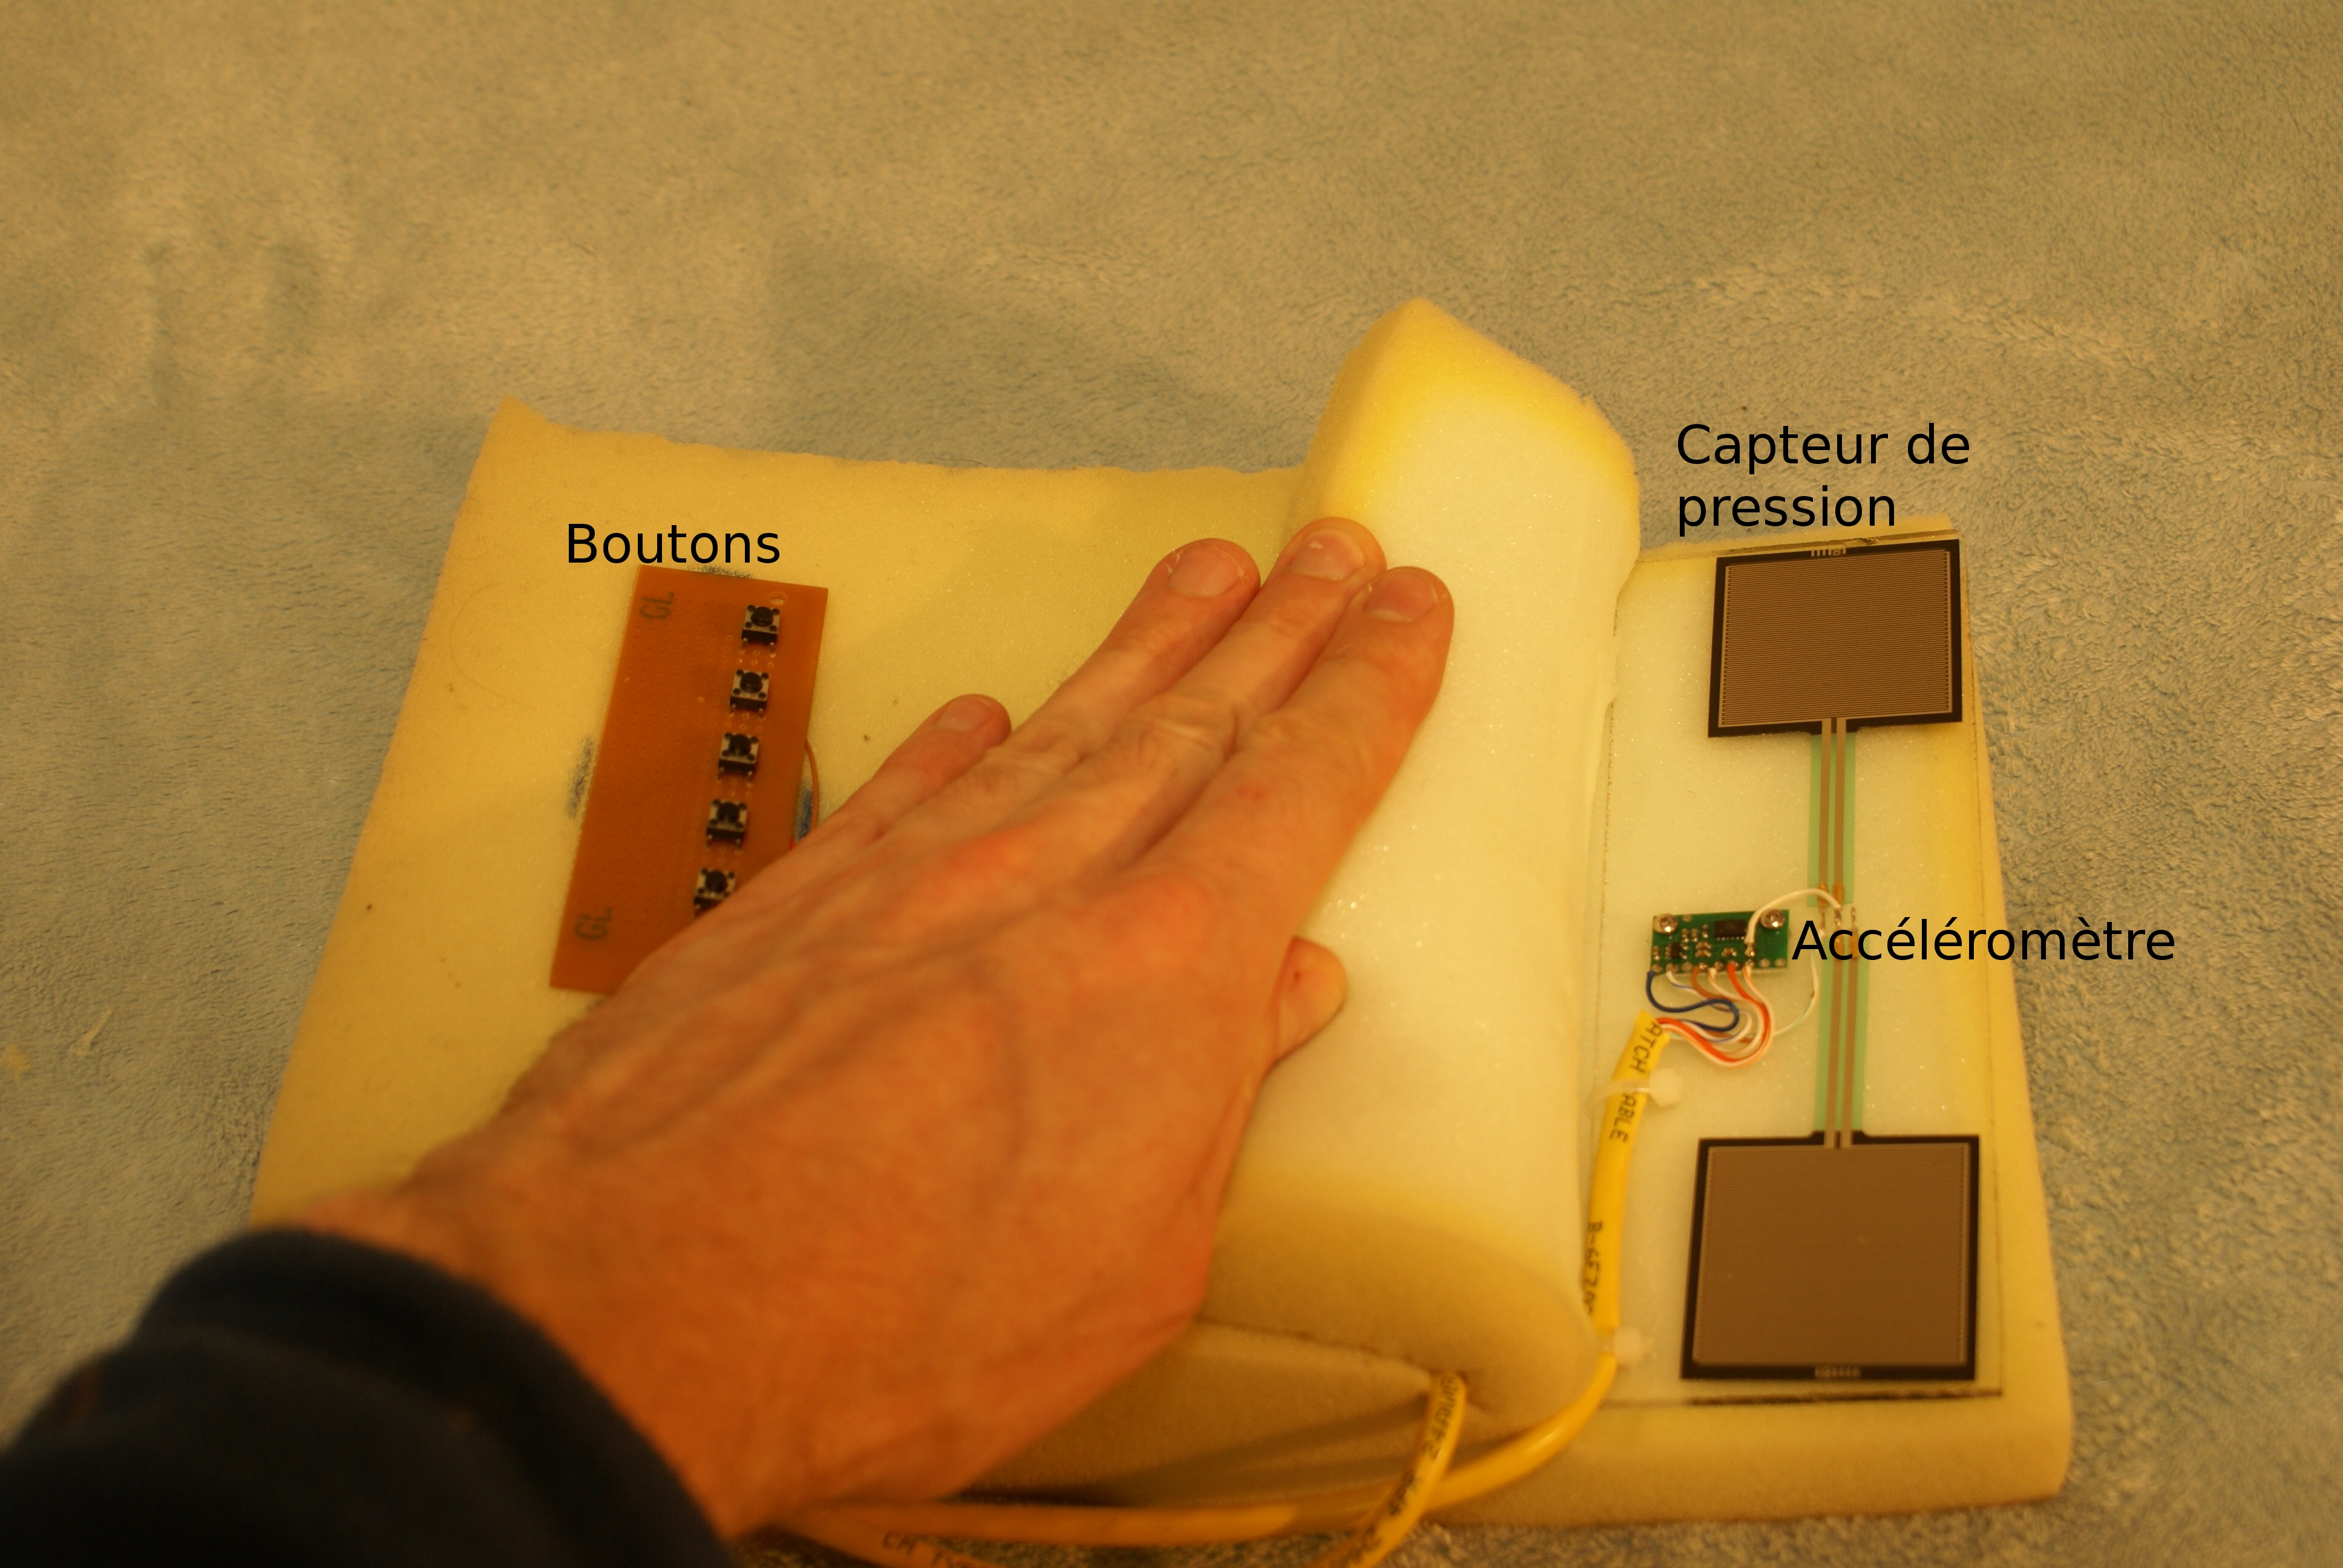
\includegraphics[height=0.14\textheight]{figs/spongeGauche.jpg}}
  \caption{L'interface musicale conçue: l'éponge.  (a) Des capteurs et un microcontrôleur.  (b) L'éponge recouverte de sa housse rayée.  (c) D'autres capteurs.}
  \label{fig:eponge}
\end{figure}


\section*{Étapes franchies}
\label{sec-2}
\subsection*{Conception de l'interface}
\label{sec-2-1}
L'interface musicale développée (l'\emph{éponge}) a fait l'objet d'une
publication \citep{Marier2010} et a été utilisée régulièrement en concert
depuis.  Elle continue de faire l'objet de modifications mineures, mais
elle a atteint une certaine maturité et est un instrument très fiable et
très expressif.
\subsection*{Mappage}
\label{sec-2-2}
Le mappage consiste à établir une correspondance entre les données des
capteurs et les paramètres du son.  Il s'agit d'une étape très délicate qui
soulève des questions fondamentales sur les nouvelles interfaces musicales
et qui, par conséquent, se situe au coeur de ce projet de
recherche-création.  De nombreuses stratégies de mappage ont été essayées
en studio et testées devant public.  Une nouvelle techniques de mappage a
été développée et a fait l'objet d'une publication \citep{Marier2012a}.  Un
second article au sujet du mappage a été soumis au \emph{Computer Music Journal}
et pourrait être publié en 2014.
\subsection*{Oeuvres}
\label{sec-2-3}
Deux oeuvres pour éponge solo ont été créées et jouées à plusieurs reprises
devant public: \emph{Clarinette (Albino Butterfly)} et \emph{L'éloge du mou}.  Ces
pièces partiellement improvisées évoluent et sont adaptées à chaque
représentation et à chaque évoluation de l'instrument.  Un autre article au
sujet du mappage, et du processus de création de ces oeuvres a été publié
\cite{Marier2012}.

\section*{Étapes prévues}
\label{sec-3}
Le travail à accomplir avant le dépôt de la thèse comporte deux volets: la
la composition d'une oeuvre pour deux éponges (un duo pour éponges) et la
conduite d'une expérience qui implique des sujets qui essaieront l'éponge.


\bibliographystyle{francais}
\bibliography{/home/marierm/Documents/mendeley/library}
% Emacs 24.3.50.1 (Org mode 8.0.3)
\end{document}